% =====================================================================
%  3.6 Hyper-parameter tuning
% =====================================================================
\subsection{Hyper-parameter Tuning}
\label{sec:tuning}

Every model is tuned on the same validation year, with validation MAE as the criterion, separately
in each weather setting. Budgets differ and are reported openly (\cref{tab:tuning}). Seed 42 is used
everywhere.

\begin{table}[H]
  \centering
  \small
  \caption{Tuning set-up.}
  \label{tab:tuning}
  \begin{tabularx}{\linewidth}{@{}l Y Y@{}}
    \toprule
    Model & Search space & Procedure \\
    \midrule
    B1 Ridge & target $\in$ \{level, change\}; $T_h\in\{10,\dots,20\}$, $T_c\in\{14,\dots,26\}$ (step
      2, $T_h\le T_c$); 11 values of $\alpha$ from $10^{-2}$ to $10^{3}$ (log scale)
      & Per target: bases at the middle $\alpha$, then $\alpha$ at the chosen bases. 94 fits per
        setting. The first $T_c$ grid started at 18 and its optimum lay on the edge, so the grid was
        widened before choosing. \\
    M1 LightGBM & target $\in$ \{level, change\}; \code{num\_leaves} 8--256; \code{min\_data\_in\_leaf}
      10--300; \code{feature\_fraction} 0.5--1; \code{lambda\_l2} $10^{-3}$--10
      & Optuna~\cite{akiba2019optuna} TPE, 30 trials. Learning rate fixed at 0.03; the number of trees
        comes from early stopping (200 rounds) on validation MAE and is kept fixed when refitting. A
        small budget on purpose: with two training years, heavy tuning overfits the validation
        year~\cite{smyl2023esdrnn}. \\
    \bottomrule
  \end{tabularx}
\end{table}

\paragraph{Ridge results.}
\Cref{tab:ridge-params} shows the chosen values. Both settings choose the change target and
$T_h=T_c=18\,^\circ$C, i.e.\ a V-shape with its minimum at 18\,$^\circ$C. The validation MAE is flat
around the optimum (all base pairs within about 30\,MW), so results do not hinge on the exact
bases. The $\alpha$ curves have an interior minimum (\cref{fig:ridge-alpha}).

\begin{table}[H]
  \centering
  \small
  \caption{Chosen Ridge hyper-parameters (validation 2017).}
  \label{tab:ridge-params}
  \begin{tabular}{@{}l l r r r r@{}}
    \toprule
    Setting & Target & $T_h$ & $T_c$ & $\alpha$ & Val.\ MAE (MW) \\
    \midrule
    actual & change & 18 & 18 & 31.6 & 1{,}839.5 \\
    lagged & change & 18 & 18 & 10.0 & 1{,}858.7 \\
    \bottomrule
  \end{tabular}
\end{table}

\begin{figure}[H]
  \centering
  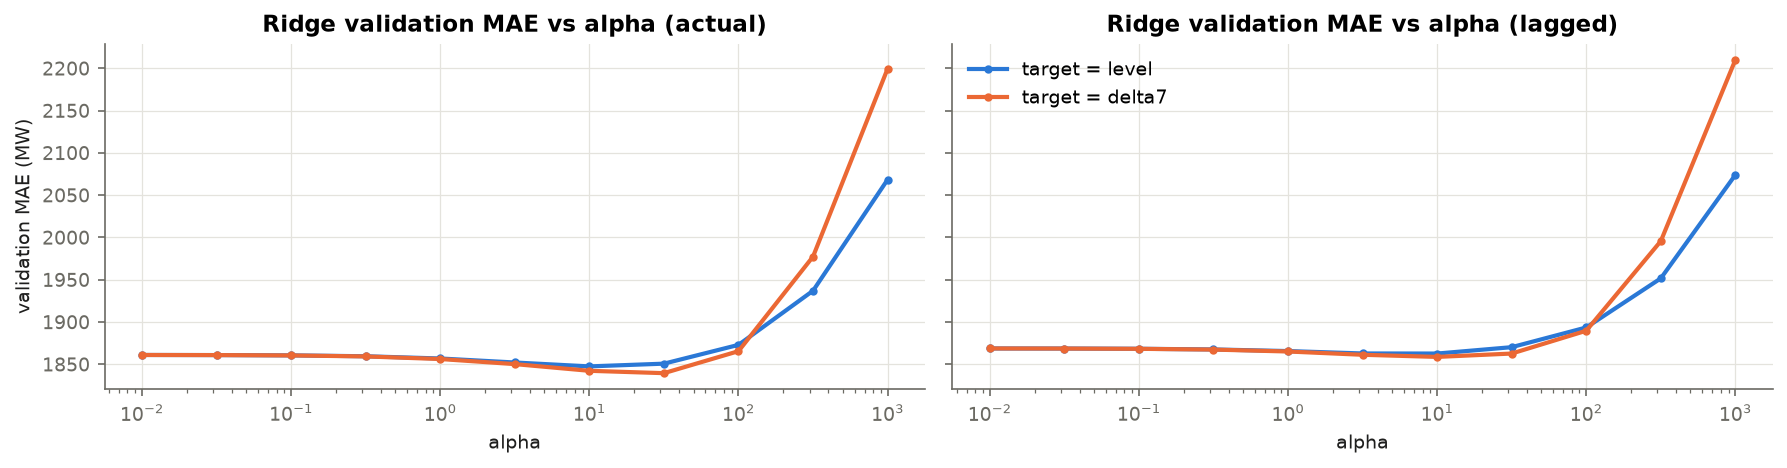
\includegraphics[width=\linewidth]{02_ridge_alpha.png}
  \caption{Ridge validation MAE against $\alpha$ for both target options.}
  \label{fig:ridge-alpha}
\end{figure}

\paragraph{LightGBM results.}
Tuning ran on a Kaggle CPU session (LightGBM 4.6.0, Optuna 5.0.0) in about 4 minutes per setting.
Both settings choose the level target: no trial with the change target came within 70\,MW of the
best level-target trial (\cref{fig:optuna}). The best-so-far curve is flat after trial 3 (actual) and trial 24 (lagged), so
30 trials are enough. The chosen models are large and lightly regularised (\cref{tab:lgbm-params}).
Because early stopping and model selection use the same validation year, the validation MAE of M1
is somewhat optimistic; the fair comparison is on the test year.

\begin{table}[H]
  \centering
  \small
  \caption{Chosen LightGBM hyper-parameters (validation 2017).}
  \label{tab:lgbm-params}
  \begin{tabular}{@{}l l r r r r r r@{}}
    \toprule
    Setting & Target & Leaves & Min.\ leaf & Feat.\ frac. & $\lambda_2$ & Trees & Val.\ MAE \\
    \midrule
    actual & level & 171 & 13 & 0.62 & 0.002 & 1{,}006 & 1{,}590.8 \\
    lagged & level & 70 & 11 & 0.55 & 0.46 & 2{,}153 & 1{,}683.4 \\
    \bottomrule
  \end{tabular}
\end{table}

\begin{figure}[H]
  \centering
  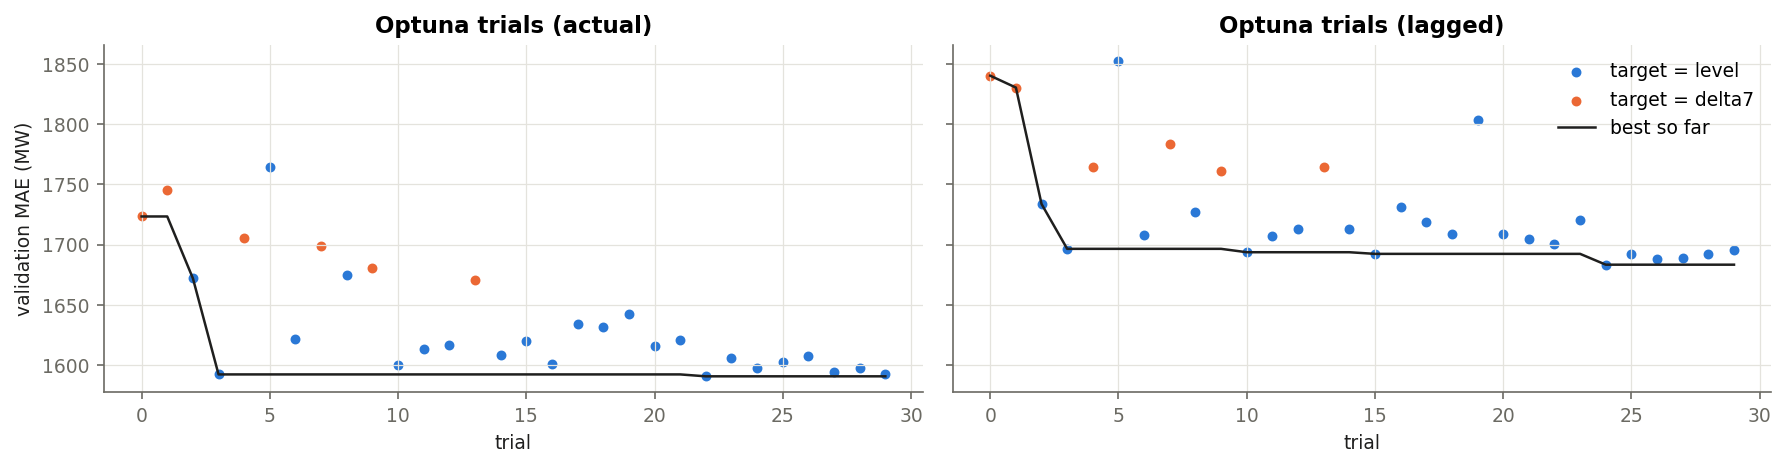
\includegraphics[width=\linewidth]{03_optuna_trials.png}
  \caption{Validation MAE of the 30 Optuna trials per setting, coloured by target option.}
  \label{fig:optuna}
\end{figure}
